\documentclass{report}
\usepackage{blindtext}
\usepackage{titlesec}
\usepackage{graphicx}
\usepackage{cite}
\usepackage{textcomp}
\usepackage{hyperref}
\usepackage{float}
\usepackage[utf8]{inputenc}
\usepackage[T1]{fontenc}
\usepackage{lmodern}
\setlength{\tabcolsep}{18pt}
\renewcommand{\arraystretch}{1.5}
\font\myfont=cmr12 at 32pt
\raggedbottom
\renewcommand\thesection{\arabic{section}}

\date{\huge 29 May, 2018 }


\begin{document}
\begin{titlepage}
    \begin{center}
        \vspace*{1cm}
        
        \Huge
        \textbf{BaahubaliStocks.com}\\
        \LARGE\textit{Stocks Aapke, Analysis Hamari}
        
        \vspace{1cm}
        \LARGE
        IIT Mandi - CS309 Information and Database Systems
        
        \vspace{1cm}
		\textbf{Group Number 1}
		
		\vspace{1cm}     
        
        \vspace{1.5cm}
        
        \textbf{The Team}
        \vspace{0.5cm}
        \large 
        
        	\begin{center}
        	\fontsize{15}{15}\selectfont
			\begin{tabular}{ c c }
			
 			Amrendra Singh & B16010 \\ 
 			Aj R Laddha & B16004 \\  
 			Sujetth Rangannath & B16036\\
 			Hritik Gupta & B16097\\ 
			\end{tabular}
			\end{center}
        
    \end{center}
\end{titlepage}


%\maketitle

\tableofcontents




\section{How to use}
\begin{enumerate}
	\item clone repo from https://github.com/ashking13th/baahubalistocks
	\item Install Django
		`sudo apt-get install python3-django`

	\item Download this repository

	\item Browse to the stocks directory in the terminal

	\item `\$ python manage.py migrate`

	\item `\$ python manage.py runserver`

	\item Go to `localhost:8080` in your browser
\end{enumerate}

\section{ Overview}
Day trading in stocks is risky, more so if you are untrained. When it comes to investing in stocks, it is important that the investor is capable of conducting a thorough technical analysis of stock charts. Technical analysis is used to define the process of forecasting future price movements based on the past price movements within stock charts. It is with the help of technical analysis that investors are able to make financial decisions of buying, holding, or selling stocks. 

By studying and evaluating past and current data, investors and traders attempts to gain an edge in the markets by making informed decisions. Such solutions and analysers are hard to find. If they exist, they cost you for the service.
BaahubaliStocks.com is a one-stop solution. Our site allows the customer to forecast which way the market is going to move and help the investor make a more financially sound investment decision. 
What all can be there?

The site will hold the historical and current trading data of stocks. It would give user the access to this raw data as well as processed data. Processed data can be like the minimum or maximum trading stock for a day, month or a year or min or max of a particular stock for a specific time frame.

Basic details of the stock like company it is linked to, all time high and low, initial offering date and price, dividend value shall be there in the details of a stock.

Background details of companies would also be there. This would keep record of all stocks linked to the company, its market value, profits, executives list among important details.

All this data can be used by our user to aid to his investment decisions.

\section{Definitions}
\subsection{User}
A customer, investor or analyst registered on our application.

\subsection{Stocks}
A stock of a particular company at an exchange

\subsection{Company} :  A company, a commercial organization which may have one or more stocks trading in its name on the stock exchange.

\subsection{Favourite} : A user will be able to ‘favourite’ certain stocks or companies for easy access to them. 

\section{Design Features}
\subsection{Login}
Users would be able to log in to our system using username and password.

\subsection{Stocks}
Stocks are the most important part. Stock prices will be stored in our database on which user can run query to get the max valued stock or the highest growing stock or the fastest growing stock which started within a specific time-frame given by the user.

\subsection{Company}
Any stock belongs to a company. A company may not be associated with a stock but all stocks shall certainly be associated with a company. User will be able to view details about a company as well as the stocks associated with it.

\subsection{Tags}
User can tag their stocks based on the companies they hold in, to get an overview of the type of stock.

\subsection{Bookmarks}
Users will be able to bookmark certain stocks that they can refer to in future.

\section{Target customer}

People who have an eye for stock markets, be it analysts, investors, venture capitals, consultants or even enthusiasts.
As of now no low cost or free service is available in the market which does such a wide variety of tasks and provide predictions from a chunk of stock market data. Most of such services are very expensive. 

The platform will serve as a tool for users who are willing to invest in stock markets or are willing to get started with the same. 
Implementation

The solution will be implemented using Django Python framework with an underlying MySQL server database.

UI would use Bootstrap and JQuery objects. Backend development would be in Python Django framework using an underlying MySQL server.
Stock data would be fetched from the raw data available with the Alpha Vantage API and process it such that we can process our queries easily and efficiently. Data would be fetched and processed regularly and then stored in our local database.

Data visualizations in the form of tables and graphs would be made possible using the python libraries. Data could be sorted in a form as per the user’s choice. 

Company details will be fetched in real time from Wikipedia.
Users will have the ability to “favorite” or in more formal terms, bookmark any stocks they find of interest which will later give them a quick access to them.

\section{ Required Hardware}
For the purpose of this project all the data will be stored on our personal computers. Because of the constraints of our PC, we will store minute by minute stock data for the last 7 days, hour by hour stock data for the last one year and day wise data for the last 10 years.

\section{Performance Requirements}
On an PC which runs on an Intel Core i5 processor with 8 GB RAM, the maximum response time for any online request must be less than 2 secs. Around 50 MB memory is used for keeping record of a 100 million entries.

\section{ ER Diagram}
An initial non normalized ER diagram for this project is attached here: 
\begin{figure}[H]
	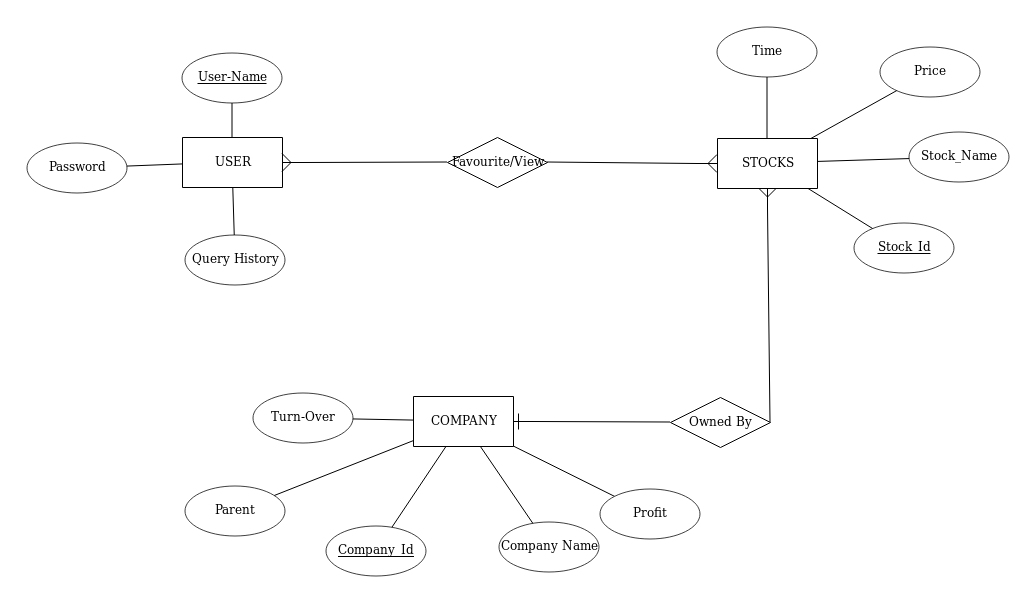
\includegraphics[scale=0.35]{erd1.png}
\end{figure}

\section{Salient Features} 
\begin{enumerate}


\item \textbf{Indexing :} We have implemented indexing on the phpMyAdmin interface, which substantially decreased our query response time, thus increasing the 
effifiency. Indexes are created on the primary key (record time), which enhanced the performance by upto 4 times.

\item \textbf{Data manipulation and prediction :} Using python modules, for instance Scipy, the data is fit into a linear regression model. The software thus predicts the 
probable stock prices for the upcoming n days.

\item \textbf{Offline Storage of Data :} We offer an efficient way to store data offline. The files can be directly downloaded by the user i.e export in the form of 
csv, in case any database corruption occurs.

\item \textbf{Query Stocks :} The software allows the user to view the analytics of a company's stocks, by searching for the company code. The interface pings back with the stock trends of the last 7 days, as well as an overview over the monthly data.

\item \textbf{Automatic updates to database:} There is a script called autoupdate.php that checks the latest recorded time of each stock and makes a call to the API to check if the stock data is up to date or not. If not, then the tables get updated.

\item \textbf{Potentially lots of data:} Some daily stock data tables have more than 3000 or 4000 records (i.e, more than past 15 years of stock data). Unfortunately, the same php script could not populate the remaining databases because of the time the free version of the API was taking to return results and due to processing limitations our normal laptops. Theroretically speaking, the php script that populated the initial few tables could also work on the rest of the tables if left running for a few days!

\end{enumerate}

\section{Performance Checks}
\subsection{Response time of API}
For a single API call the response time is around 1.5 to 2 seconds. Interestingly enough, his is
irrespective of the amount of data transferred after the call.
\subsection{Time for query execution}
Here are some results that indicate response time with various kinds of indexing. These have been performed on the data of a stock called ‘ABB’. The name of the table is abbdaily.

\begin{itemize}

\item “SELECT MIN(value) FROM abbdaily”
-Took 0.0024 seconds without index on ‘value’ and 0.0017 with index\\

\item “SELECT MIN(value) FROM abbdaily WHERE recordtime BETWEEN '2005-03-03' AND '2013-03-03'”\\
 -0.0038 seconds without index on value and 0.0031 seconds with index\\
 
\item “SELECT * FROM abbdaily WHERE recordtime = ‘2010-05-05’”\\
0.0028 seconds without index on recordtime and 0.0006 seconds with index\\

\item “SELECT * FROM abbdaily WHERE value = 22”\\
0.0026 seconds without index on value and 0.0007 seconds with index\\

\item “SELECT * FROM abbdaily WHERE recordtime > '2010-05-05' ORDER BY value DESC”\\
-No index : 0.0035 seconds\\
-Index on primary key: 0.0018 seconds [Index on recordtime]\\
-Index on value: 0.0032 seconds\\
-Index on (recordtime, value) : 0.0022 seconds\\
-Index on (value, recordtime) : 0.0011 seconds\\


\end{itemize}

\subsection{Time for loading graph}
It takes less than one second to display the graph.
Note that these values are noted when the queries ran our local machines and therfore does not
account for the delay networks may induce.

\subsection{API}
Due to bad performance of API, scripts running on the server making use of the API take several tens of seconds to run. For instance the autoupdate.php took almost 60 seconds to update records in the first two tables of the database. 4300 records were updated so the time taken for that also has to be factored in.

\section{Amount of Data}
A script was used to extract stock symbol data from a website(ref - http://www.marketonmobile.com/search.php). The API requires symbols so only the NSE symbols were extracted. Even among these symbols, the API did not support certain stocks. A script was written to eliminate all such stocks. After that, there were aroundd 1300 stocks left. For each of these stocks two tables were created. One table for storing the daily data and one more to store the monthly data. The first ten or so daily stock tables were fully populated and had an average of 3000 tuples. The rest of the daily tables made use of a light version of the API call and had 100 tuples each. The first 50 or so monthly tables had 100 tuples each.
With only these few tables at the beginning there are already 70,000 tuples in total. There are still around 2000 tables that are yet to be populated.

Once that is done, the total number of tuples is estiated to be over 30,00,000. The space occupied is estimated to ber over 700 MB. Also keep in mind that as of now, the tuples only have a record date and a stock price. There are many other parameters in stock marketing and adding them could easily make the size to go over many gigabytes of data!

\section{Problems Faced}
\begin{itemize}
	\item The API call is extremely slow when used with PHP. Sometimes it takes tens of seconds for us to get the result. 
	\item In general the free version of the API is extremely unstable. It sometimes gives an error message as the JSON output when too many function calls are made in limited period of time. Due to this it was very difficult to populate the databases.
\end{itemize}

\section{Future Scope}
The same project can be extended to have a lot of different kind of values. Right now in each table we only have the record date and the closing price on that day. We can even add volume of stock, opening price etc. and run queries on all this data. 

We can definitely do a better job at populating the tables though that would probably cost us some money and not to mention, a better laptop maybe required to do it in less time.

A more sophisticated interface to execute user queries must be though of and implemented. 

Right now, the autoupdate.php script for updating stock data needs to be run manually by the user but in a server environment, a bash script to periodically execute the same PHP file can easily be made.

A more complicated machine learning model taking into account various stock parameters other than just the price can be implemented making it a full fledged stock market predictor

\section{Conclusion}
BaahubaliStocks.com would be handy tool for thousands of people including investors and stock market enthusiasts to serve their purpose without spending a single buck, developed using Django, MySQL, HTML5, Bootstrap and JQuery on top of Alpha Vantage API and Python libraries. 



\begin{thebibliography}{00}
\bibitem{amazongo} Django \\
	\textit{\url{https://www.djangoproject.com/}} \\
	
\bibitem{rfidwiki} Bootstrap \\
	\textit{\url{http://getbootstrap.com/}}

\bibitem{facewiki} Alpha Vantage \\
	\textit{\url{https://www.alphavantage.co/documentation/}}
	

\end{thebibliography}

\end{document}